\documentclass{article}
\usepackage[utf8]{inputenc}
\usepackage{amsmath, amssymb, amsthm, cancel}
\usepackage{enumitem}
\usepackage{caption}
\usepackage{graphicx}
\usepackage[top=1in, bottom=1in, left=1in, right=1in]{geometry}
\usepackage{float}
\usepackage{booktabs}
\usepackage{array}
\usepackage{multirow}

\title{\textbf{CSCI4150U: Data Mining}\\K-Means and Hierarchical Clustering}
\author{Syed Naqvi \\ Student ID: 100590852}
\date{\today}

\begin{document}

\maketitle

\begin{abstract}
This report analyzes K-means and Hierarchical clustering on the Breast Cancer Wisconsin and Waveform datasets, using Sum of Squared Errors
(SSE) as a metric and the elbow method for k-means model selection. Hierarchical clustering methods (Single, Complete, and Group Average
Link) are visualized using dendrograms. Findings show K-means effectively identifies natural groupings in the data and Hierarchical
clustering confirms these groupings by revealing a significantly reduced rate of inter-cluster distance reductions beyond optimal
partitioning. The report highlights the effectiveness of K-means and Hierarchical clustering algorithms in finding natural data clusters.
\end{abstract}
    
    

\section{Introduction}

\subsection{Methodology}
Datasets used in this analysis are sourced from the \textit{UC Irvine Machine Learning Repository} and include:
\begin{itemize}
    \item \textbf{Breast Cancer Wisconsin (Diagnostic)}
    \item \textbf{Waveform Database Generator (Version 1)}
\end{itemize}

We evaluate the following clustering algorithms:
\begin{itemize}
    \item \textbf{K-means Clustering}
    \item \textbf{Hierarchical Clustering} (Single Link, Complete Link, and Group Average)
\end{itemize}

For K-means clustering, model \( k \) values range from 1 to 6 for the \textit{Breast Cancer Wisconsin (Diagnostic)} dataset
and 2 to 6 for the \textit{Waveform Database Generator (Version 1)} dataset. Clustering performance is assessed using the Sum of Squared Errors
(SSE) with Euclidean distance as the metric.

\newpage

\subsection{Preprocessing}
To perform accurate clustering, we analyze feature ranges to determine the dataset most needing of standardization.
\begin{figure}[H]
    \centering
    \begin{minipage}[b]{0.49\textwidth}
        \centering
        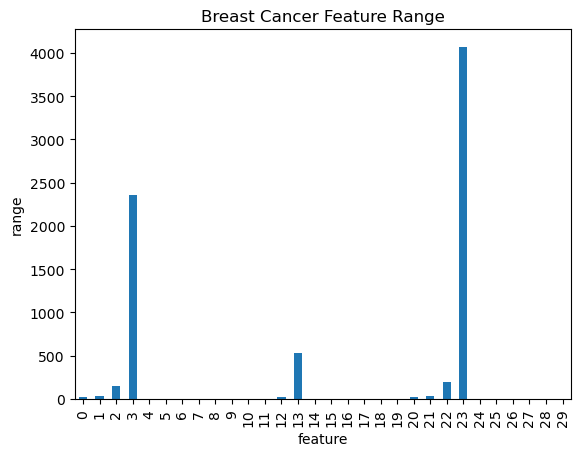
\includegraphics[width=\textwidth]{p_i.png}
        \caption{Pre-Standardized Feature Ranges (Breast Cancer Data)}
    \end{minipage}
    \hfill
    \begin{minipage}[b]{0.49\textwidth}
        \centering
        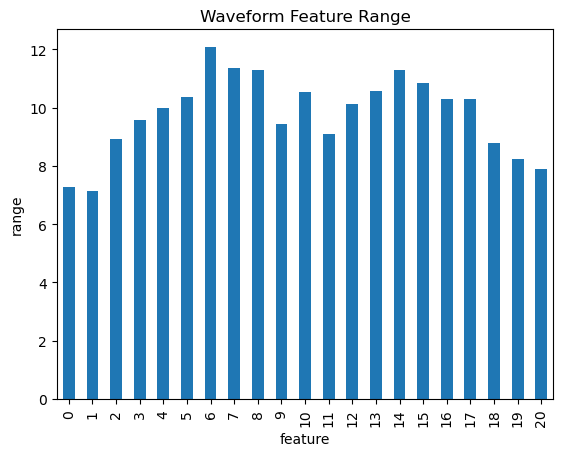
\includegraphics[width=\textwidth]{p_ii.png}
        \caption{Pre-Standardized Feature Ranges (Waveform Data)}
    \end{minipage}
\end{figure}
\begin{figure}[H]
    \centering
    \begin{minipage}[b]{0.49\textwidth}
        \centering
        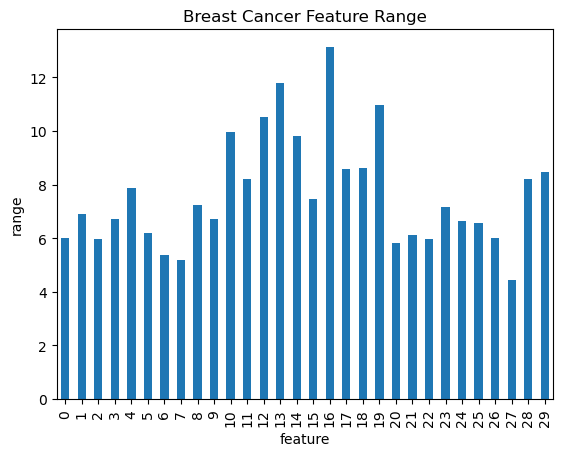
\includegraphics[width=\textwidth]{p_iii.png}
        \caption{Post-Standardized Feature Ranges (Breast Cancer Data)}
    \end{minipage}
    \hfill
    \begin{minipage}[b]{0.49\textwidth}
        \centering
        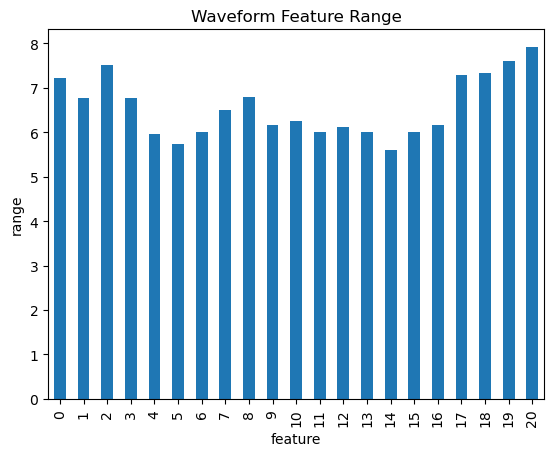
\includegraphics[width=\textwidth]{p_iv.png}
        \caption{Post-Standardized Feature Ranges (Waveform Data)}
    \end{minipage}
\end{figure}

The feature values have now been scaled and are significantly better suitable for clustering. 

\newpage

\section{Part I: K-Means Clustering}
\subsection{Model Selection}
\begin{figure}[H]
    \centering
    \begin{minipage}[b]{0.49\textwidth}
        \centering
        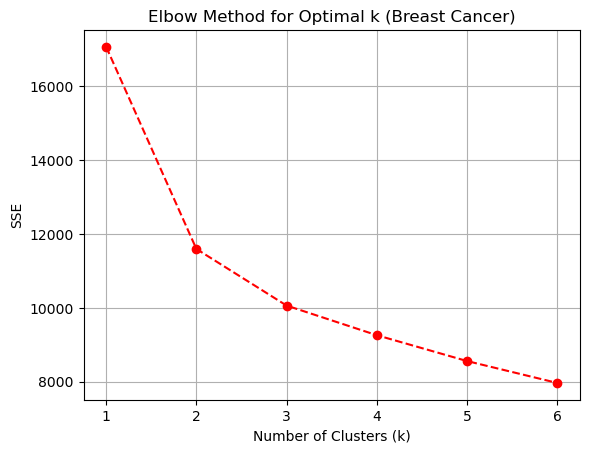
\includegraphics[width=\textwidth]{elbow_cancer.png}
        \caption{Elbow method for selecting optimal K-value (Breast Cancer Dataset)}
    \end{minipage}
    \hfill
    \begin{minipage}[b]{0.49\textwidth}
        \centering
        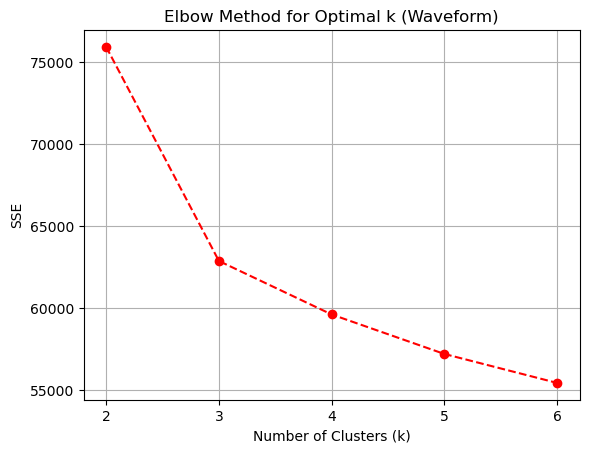
\includegraphics[width=\textwidth]{elbow_waveform.png}
        \caption{Elbow method for selecting optimal K-value (Waveform Dataset)}
    \end{minipage}
\end{figure}

From the above figures, the ideal number of clusters is \textbf{k=2} for the Breast Cancer dataset and \textbf{k=3} for the Waveform dataset. This
suggests there are likely 3 distinct waveforms in the Waveform dataset and two distinct tumor categorizations (malignant or benign)
in the Breast Cancer dataset which is of course consistent with the actual number of unique labels in both datasets.

\subsection{Results}

Using the ideal cluster amounts for each dataset, the following tables display centroids with lowest SSE scores achieved through
convergence with a maximum of 300 iterations and 10 rounds of unique seed placement.
\begin{figure}[H]
    \centering
    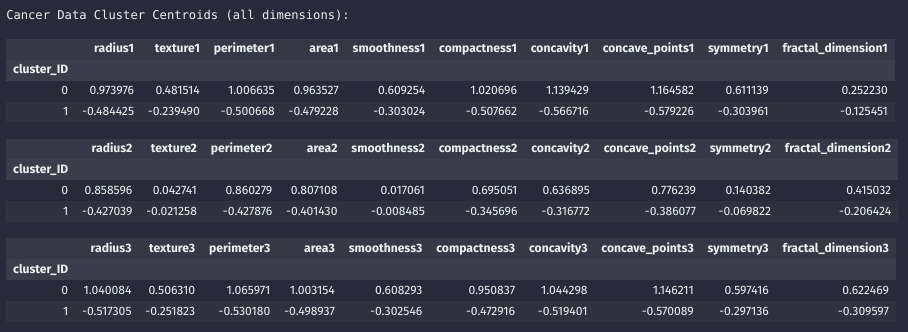
\includegraphics[width=\textwidth]{cancer_centroids.png}
    \caption{Centroids (Breast Cancer Dataset)}
\end{figure}
\begin{figure}[H]
    \centering
    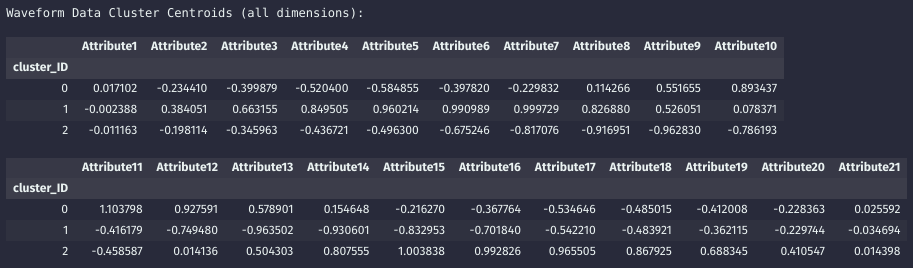
\includegraphics[width=\textwidth]{waveform_centroids.png}
    \caption{Centroids (Waveform Dataset)}
\end{figure}

Using Euclidean distance as our metric, we can view the top five closest points in each cluster to their centroid across both datasets.
\begin{figure}[H]
    \centering
    \begin{minipage}[b]{0.47\textwidth}
        \centering
        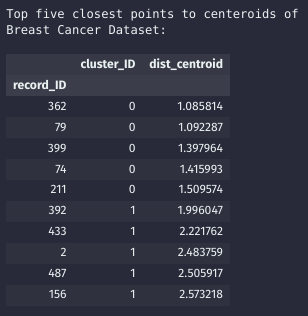
\includegraphics[width=\textwidth, height=0.3\textheight]{top_five_cancer.png}
        \caption{Top five closest points to their cluster centroids (Breast Cancer Dataset)}
    \end{minipage}
    \hfill
    \begin{minipage}[b]{0.47\textwidth}
        \centering
        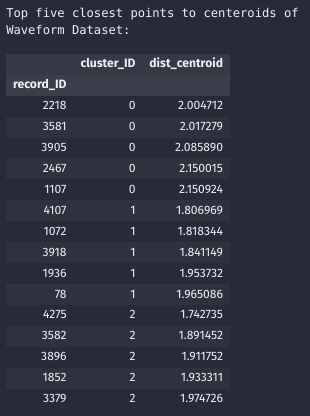
\includegraphics[width=\textwidth, height=0.3\textheight]{top_five_waveform.png}
        \caption{Top five closest points to their cluster centroids (Waveform Dataset)}
    \end{minipage}
\end{figure}

\newpage

\section{Part II: Clustering Task}

Next, we use dendrograms to visualize the Single Link, Complete Link and Group Average forms of Hierarchical clustering. We truncate the
graphs above 30 separate clusters and visualize when the various distance metrics seems to converge.

\begin{figure}[H]
    \centering
    \begin{minipage}[b]{0.49\textwidth}
        \centering
        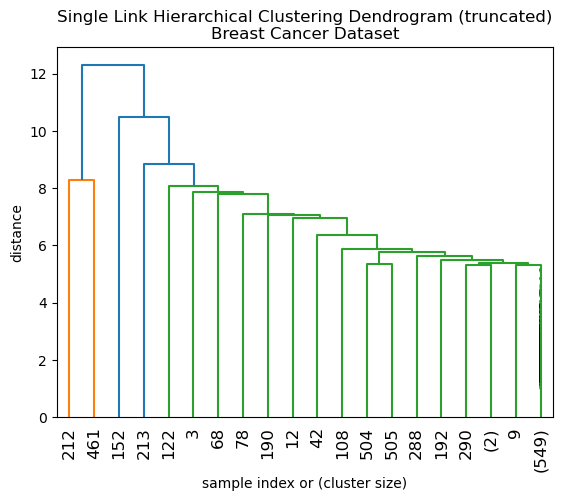
\includegraphics[width=\textwidth, height=0.3\textheight]{single_cancer_dend.png}
        \caption{Single Link Hierarchical Clustering (Breast Cancer Dataset)}
    \end{minipage}
    \hfill
    \begin{minipage}[b]{0.49\textwidth}
        \centering
        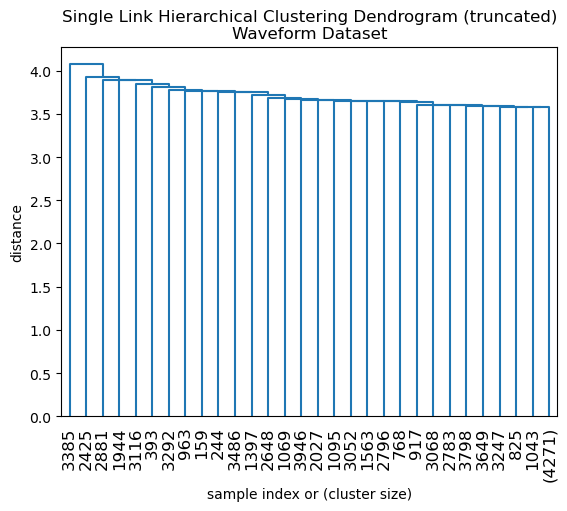
\includegraphics[width=\textwidth, height=0.3\textheight]{single_waveform_dend.png}
        \caption{Single Link Hierarchical Clustering (Waveform Dataset)}
    \end{minipage}
\end{figure}
\begin{figure}[H]
    \centering
    \begin{minipage}[b]{0.49\textwidth}
        \centering
        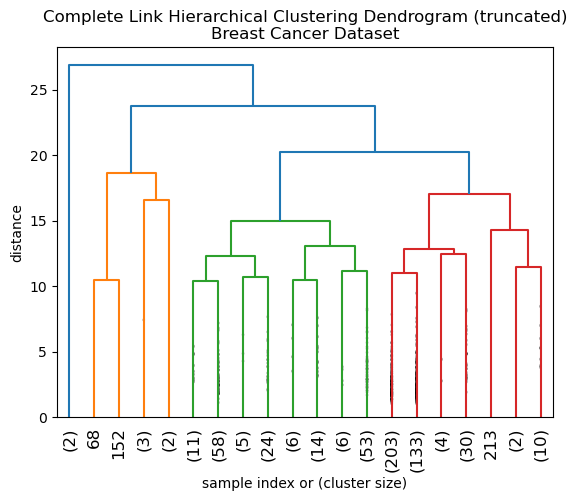
\includegraphics[width=\textwidth, height=0.3\textheight]{complete_cancer_dend.png}
        \caption{Complete Link Hierarchical Clustering (Breast Cancer Dataset)}
    \end{minipage}
    \hfill
    \begin{minipage}[b]{0.49\textwidth}
        \centering
        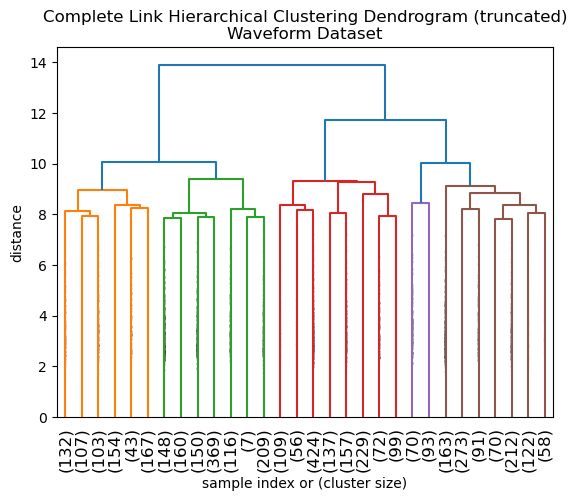
\includegraphics[width=\textwidth, height=0.3\textheight]{complete_waveform_dend.png}
        \caption{Complete Link Hierarchical Clustering (Waveform Dataset)}
    \end{minipage}
\end{figure}
\begin{figure}[H]
    \centering
    \begin{minipage}[b]{0.49\textwidth}
        \centering
        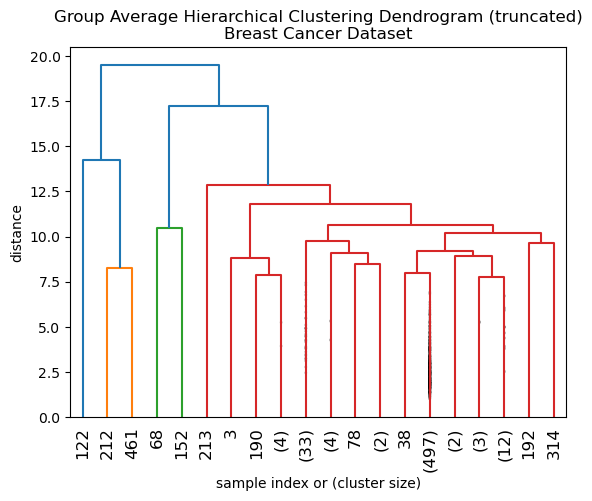
\includegraphics[width=\textwidth, height=0.3\textheight]{average_cancer_dend.png}
        \caption{Group Average Hierarchical Clustering (Breast Cancer Dataset)}
    \end{minipage}
    \hfill
    \begin{minipage}[b]{0.49\textwidth}
        \centering
        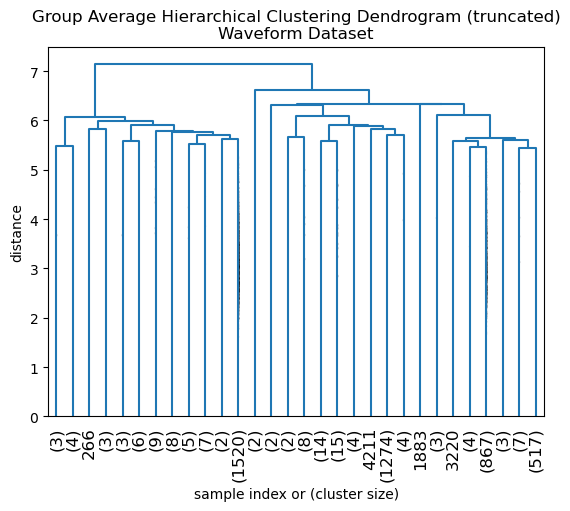
\includegraphics[width=\textwidth, height=0.3\textheight]{average_waveform_dend.png}
        \caption{Group Average Hierarchical Clustering (Waveform Dataset)}
    \end{minipage}
\end{figure}


\section{Conclusion}
This report demonstrates that both K-means and hierarchical clustering methods effectively identify natural groupings given relatively
simpler and small datasets. Using Sum of Squared Errors (SSE) and the "elbow method" for optimal \( k \)-selection, the K-means algorithm
can effectively identify natural groupings in the data while the Single Link, Complete Link and Group Average Hierarchical clustering
variants further corroborate these groupings through dendrogram visualizations. These visualizations reveal significantly reduced
\textit{rate of reduction} in inter-cluster distance beyond a certain level of partitioning, indicating a natural stopping point for
clustering. Overall, the analysis highlights the complementary strengths of K-means and hierarchical clustering in data mining tasks.

\end{document}
